%% LyX 1.1 created this file.  For more info, see http://www.lyx.org/.
%% Do not edit unless you really know what you are doing.
\documentclass[english]{report}
\usepackage[T1]{fontenc}
\usepackage[latin1]{inputenc}
\usepackage{geometry}
\geometry{verbose,a4paper}
\usepackage{babel}
\usepackage{graphics}

\makeatletter

%%%%%%%%%%%%%%%%%%%%%%%%%%%%%% LyX specific LaTeX commands.
\providecommand{\LyX}{L\kern-.1667em\lower.25em\hbox{Y}\kern-.125emX\@}
%% Special footnote code from the package 'stblftnt.sty'
%% Author: Robin Fairbairns -- Last revised Dec 13 1996
\let\SF@@footnote\footnote
\def\footnote{\ifx\protect\@typeset@protect
    \expandafter\SF@@footnote
  \else
    \expandafter\SF@gobble@opt
  \fi
}
\expandafter\def\csname SF@gobble@opt \endcsname{\@ifnextchar[%]
  \SF@gobble@twobracket
  \@gobble
}
\edef\SF@gobble@opt{\noexpand\protect
  \expandafter\noexpand\csname SF@gobble@opt \endcsname}
\def\SF@gobble@twobracket[#1]#2{}

\makeatother
\begin{document}

\title{\textbf{Brainstorm}}


\author{ObliVion}

\maketitle

\subsubsection*{Trademarks}

Product names used in this publication are for identification purposes
only and may be trademarks of their respective companies

\tableofcontents{}


\chapter{aMOS}

The goal of aMOS is to be as versatile as possible, meaning that it
should adjust itself to the users needs. This goal has a lot of disadvantages
compared to a more task-oriented approach. One of them, that there
is a lot of end-user decisions when installing the OS. There are some
examples of very complex OSes on the marked, that hide a lot of details
from the user behind a pretty GUI. The simple idea behind aMOS is
that the user knows best, therefore nothing will be hidden unless
the user specifies it. 

This means that aMOS will have to {}''grade{}'' the user when installing
itself, and ultimately learn what level the user is on, by watching
the user in action. The goal of monitoring the user, and adapting
to his needs, is as I see it a very complex task involving some kind
of intelligence in aMOS. This intelligence could then extend to handling
and recovering from crashes, and best of all see to it that they never
happen again.

Another feature that helps recovering from a crash, that every object
in aMOS is required to save the last functioning state, and figure
out what went wrong between then and the crash, and then gracefully
recover.

Both of these features may require a lot of processing power, for
monitoring, and a lot of space for saving the safe states of the objects
of aMOS.


\section{The general design}

The idea is to make aMOS as object oriented as possible, even though
in this early stage everything is coded in ANSI C. The reason for
choosing ANSI C is that the C library is easier to implement, and
at this stage where no binary object format has been defined, and
no compilers ported, there are some difficulties with RTTI\footnote{%
Run-Time Type Information
}. \textbf{Just keep in mind that the code is destined to a complete
rewrite in C++, and therefore keep things as object oriented as possible.}

There are some properties that every object in the system need to
implement to be accepted as a liable system component:

\begin{itemize}
\item At least one mailbox
\item The ability to tell other objects about its capabilities through this
mailbox
\item Rules regarding what system compenents it may access
\item Denial of unauthorized request
\end{itemize}

\chapter{\emph{The BOSS}\footnote{%
Basic Operating System Services
} \emph{kernel}}


\section{The design}

The BOSS kernel is a system dependent micro kernel, that export a
default functionality no matter the features of the underlying hardware.
It is the lowest level of abstraction from the hardware of the target
system, and the base of aMOS. The level of functionality that the
BOSS kernel provides, is enough for running a usable shell thereby
creating a very simple OS, but the intended use of the BOSS kernel,
is as the base component in an operating system, that extend the services
provided by the BOSS kernel.

The goal of the BOSS kernel is to export the features found on the
target machine, without breaking the limits of the BOSS specifications,
thereby creating the base for an architecture independent OS. This
is accomplished by allowing the basic framework of the BOSS kernel
to be extended by adding modules to the fundamental classes of services.
These modules are registered as subcomponents of the service class.
For instance on the Intel x86 platform the memory manager will have
a subcomponent for managing virtual memory, since the processor support
these extensions.

The BOSS kernel export all of its services through an IPC\footnote{%
Inter-Process Communication
} system that uses mailboxes. By using the IPC system as the only means
of requesting services from the BOSS kernel protection of the internals
of BOSS are greatly simplified, due to the fact that the BOSS compenents
has complete control when it comes to granting to access its services. 


\begin{figure}[!htbp]
{\centering 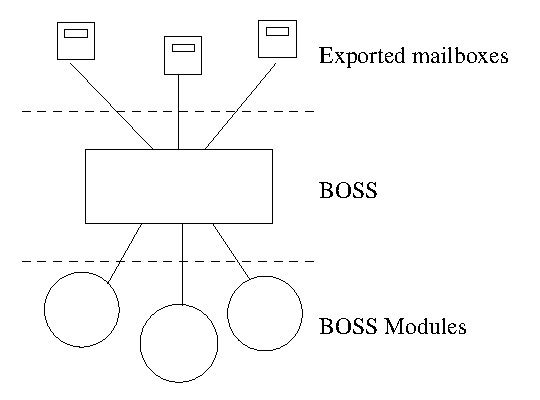
\includegraphics{BOSS_design.eps} \par}


\caption{\label{fig:BOSSdes}The BOSS kernel design}
\end{figure}


Looking at figure \ref{fig:BOSSdes} you will see that the idea behind
the BOSS kernel is the same as the HAL\footnote{%
Hardware Abstraction Layer
} in Windows NT, except for the fact that HAL told Dave, that his mind
was going. Abstracting the hardware from the rest of the OS is a very
good design decision, the problem with HAL, from my point of view,
was that the drastic limitations on hardware access slowed certain
task. I am thinking about the multimedia related features of the OS,
but the point of Windows NT, I think, has never been to provide blazing
speed for multimedia applications. The goal of Windows NT was to create
a stable fault tolerant OS suitable for companies in need of a good
OS with a nice user interface.

Relying on an IPC system 


\subsection{Hardware interface}

The BOSS has direct access to all parts of the hardware on the target
machine, but may only utilize this hardware for the sake of providing
the default functionality. The BOSS kernel provide the module mechanism
to extend the basic functionality, and take advantage of special hardware
capabilities\textbf{. The BOSS kernel should be designed to run on
the target architecture with no modules loaded, so that the basic
services may be provided, in case of system failure.} The BOSS may
implement features that are beyond standard functionality if needed.
For instance the Intel x86 version will have a virtual memory system
as default because it makes loading of modules easier. These extended
capabilities will still have the look of an extension module to the
layers running on top of the BOSS kernel.

If there are no modules loaded, the BOSS kernel will use its own standard
implementation to gain access to the hardware features of the system.
Modules provide optimizations for the rest of the system, modules
are loaded to provide better utilization of the features of for instance
the CPU, of the system. 

\vspace{0.3cm}
{
\begin{figure}[!htbp]
{\centering 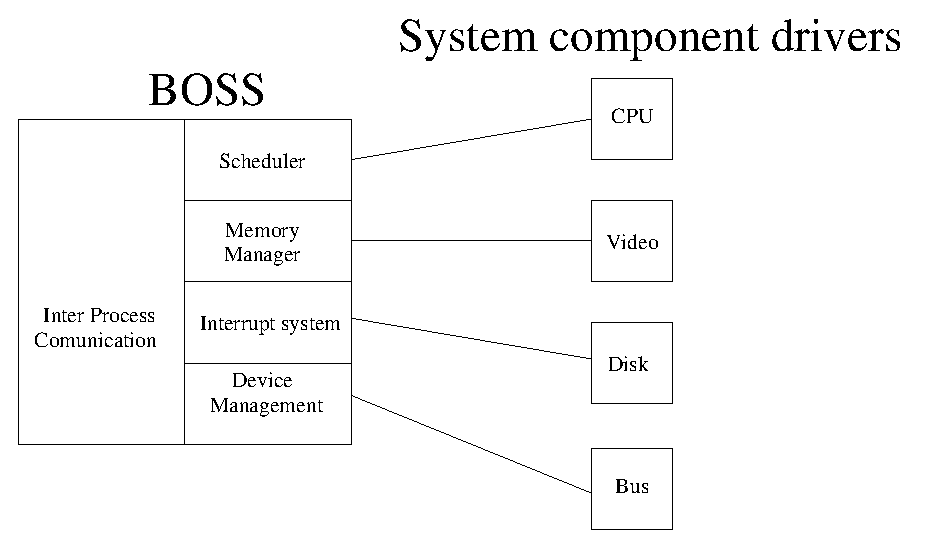
\includegraphics{BOSS_hi.eps} \par}


\caption{The BOSS kernel hardware interface}
\end{figure}
\par}


\subsection{BOSS interface}

The BOSS kernel uses an Interprocess Communication (IPC) system to
export a default functionality. Every service provided by the BOSS
kernel has a mailbox, through which communication takes place. Basically
this is what BOSS exports:

\begin{itemize}
\item A \emph{send} function for sending a message to a specific mailbox
\item A \emph{get\_mb\_desc} to acquire a handle for a mailbox
\end{itemize}

\section{The BOSS kernel functionality}

The BOSS kernel has a well defined default functionality. \textbf{It
is required that the target system is able to provide a hardware base,
that makes it possible for the BOSS kernel to export this default
functionality}, \textbf{}either trough direct use of the hardware,
or through emulation of the missing components on top of the hardware
present. The default functionality consist of the following components:

\begin{itemize}
\item A console
\item Memory management
\item Scheduling and multitasking
\item Protection
\item IPC
\item Interrupt control
\item Character device control
\item Block device control
\end{itemize}
Services from the BOSS kernel are called upon, by sending a query
message to the mailbox of the service. This makes the IPC the heart
of the BOSS kernel, and isolates the location of the BOSS kernel from
the caller, enforcing some level of protection from malicious software.
All of the exported services can have extension, provided by special
mailboxes. The exact capabilities of these extensions can be investigated
using the root service's mailbox.
\begin{figure}[!htbp]
{\centering \includegraphics{ext_examp.eps} \par}


\caption{Example of service extensions}
\end{figure}



\subsection{The console}

The console should be thought of as a special kind of the character
devices mentioned later. It is the device that has been used to display
status messages since the BOSS kernel was initialized. This device
is guaranteed to stay put until the BOSS has shutdown its services.
On a PC system this is usually some kind of video adapter, but this
can be any kind of device, that is able to print characters; It could
be a text file on disk. \textbf{The BOSS kernel implementation can
choose to provide only a dummy driver for the console}, \textbf{}so
that the messages to this output are send into oblivion.


\subsubsection{Memory management}

The BOSS kernel export the following functions for memory management:

\begin{itemize}
\item Get total system memory
\item Get map of allocated areas and their use
\item Allocate a block of memory
\item Deallocate a block of memory
\item Rules for handling allocation of special memory blocks like DMA and
such
\end{itemize}
The memory management facilities of the BOSS kernel is for basic allocation
only. It is designed to allocate large blocks of memory. and is not
very fast, so lots of allocation/deallocation cycles is simply a waste
of time. The idea is to extend this memory manager by allocating a
block of memory, and letting a more specific memory allocator manage
that specific block. This means thatSpecial blocks like DMA-buffer
and the like, are handled by this allocator.


\begin{figure}[!htbp]
{\centering \includegraphics{mm_aloc_example.eps} \par}


\caption{}
\end{figure}



\subsection{Scheduling and multitasking}

The BOSS kernel export the following functions for scheduling and
multitasking:

\begin{itemize}
\item Create / destroy a task
\item Sleeping tasks
\item \textbf{Scheduling policy yet unknown}
\end{itemize}

\subsubsection{Protection}


\subsubsection{IPC}


\section{Modules}

A module is an entity in the system dedicated to a certain task, this
may be a process scheduler, a disk driver, etc. The module format,
specifies a subset of the aMOS object format specificaly used from
the BOSS kernel and upwards. 

\vspace{0.3cm}
{
\begin{figure}[!htbp]
{\centering 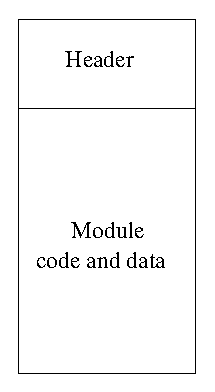
\includegraphics{module_basic.eps} \par}


\caption{Structure of a module}
\end{figure}
\par}
\vspace{0.3cm}


\subsection{Module header}

The module header contain initial information needed by the BOSS kernel
to load and initialize its services.

\begin{itemize}
\item \emph{magic number} is a special number starting at the very first
byte in the file, telling that this really is a module
\item \emph{header size} is the size of the header data structure at the
start of the module
\item \emph{validation ID} is and MD5\cite{MD5} key generated from the
code sections in the file, and is used to check if the module has
been tampered with.
\item \emph{32/64 bit module} is used to tell whether this module is for
32 or 64 bit architectures
\item \emph{section table offset} the offset, from the beginning of the
file, where the section table is located
\item \emph{section table entries} teth number of sections there are in
the section table
\end{itemize}
The structure looks like this in C:

\texttt{~}

\texttt{struct module\_header}

\texttt{\{}

\texttt{~~~~~~~~char~~~~~~~~~~~~mh\_magic{[}10{]};}

\texttt{~~~~~~~~unsigned long~~~mh\_size;}

\texttt{~~~~~~~~unsigned long~~~mh\_id{[}2{]};}

\texttt{~~~~~~~~unsigned long~~~mh\_st\_offset;}

\texttt{~~~~~~~~unsigned long~~~mh\_st\_entries;}

\texttt{\}}


\subsubsection{Magic number}

The magic number is found at posistion 0 and it is used to identify
the file as a valid aMOS module. The magic number consist of the chars
{}''\texttt{aMOSmodule}{}'' in 8-bit ASCII format which gives this
byte sequence 

\texttt{0x61 0x4d 0x4f 0x53 0x6d 0x6f 0x64 0x75 0x6c 0x65.}


\subsubsection{Header size}

This entry simply tells the size of the whole header


\subsubsection{Validation ID}

This is a 64 bit key generated by applying the MD5\cite{MD5} algorithm
to all the code sections in the module file. The code sections are
processed in the the same order as they are mentioned in the section
table. This value is used to check if the code of the module is still
intact.


\subsubsection{32/64 bit module}

This is a byte value of either 32 or 64 telling if the module is targeted
at a 32 or 64 bit architectures.


\subsubsection{Section table offset}

The byte offset from the start of the file, where the section table
is to be found. The section table is futher described in \ref{Section tables}.


\subsection{\label{Section tables}Section table}


\subsection{aMOS Interface Definition files}

\texttt{<interface>}

\texttt{~~~~~~~~name=\char`\"{}intr\char`\"{}}

\texttt{~~~~~~~~manager=\char`\"{}BOSS\char`\"{}}

\texttt{~~~~~~~~mailbox=\char`\"{}/dev/intr\char`\"{}}

\texttt{~~~~~~~~description=\char`\"{}Low level interrupt
control\char`\"{}}

\texttt{~~~~~~~~<provides>}

\texttt{~~~~~~~~~~~~~~~~BOSS.interrupt.low\_level}

\texttt{~~~~~~~~</provides>}

\texttt{~~~~~~~~<depends>}

\texttt{~~~~~~~~~~~~~~~~BOSS.ipc}

\texttt{~~~~~~~~~~~~~~~~BOSS.mm}

\texttt{~~~~~~~~</depends>}

\texttt{~~~~~~~~<exports>}

\texttt{~~~~~~~~~~~~~~~~int~~~~~~~~~~~~~n\_intr~~\#
Number of interrupts}

\texttt{~}

\texttt{~~~~~~~~~~~~~~~~func~~~~int~~~~~init(void)}

\texttt{~~~~~~~~~~~~~~~~func~~~~int\_shutdown(void)}

\texttt{~}

\texttt{~~~~~~~~~~~~~~~~msg~~~~~~~~~~~~~MSG\_INT\_<unsigned
long>}

\texttt{~~~~~~~~~~~~~~~~msg~~~~~~~~~~~~~MSG\_HOOK\_INT}

\texttt{~~~~~~~~</exports>}

\texttt{</interface>}

~

~

~




\section{Implementation example (I386)}

\begin{thebibliography}{MD5}
\bibitem[MD5]{MD5}Request for Comments 1231\end{thebibliography}

\end{document}
